\documentclass[9pt, letterpaper, landscape]{article}
\usepackage[utf8]{inputenc}
\usepackage[T1]{fontenc}
\usepackage[margin=0.3in, top=0.5in, bottom=0.4in]{geometry}
\usepackage{amsmath, amssymb, bm, amsthm}
\usepackage{tikz}
\usetikzlibrary{calc, shapes.geometric, shadows.blur, positioning, arrows.meta, matrix, decorations.pathreplacing, 3d, perspective}
\usepackage{tikz-3dplot}
\usepackage{animate}
\usepackage[most]{tcolorbox}
\usepackage{multicol}
\usepackage{ebgaramond}
\usepackage{titlesec}
\usepackage{fancyhdr}
\usepackage{tabularx}
\usepackage{booktabs}
\usepackage{pgfplots}
\pgfplotsset{compat=1.18}
\usepgfplotslibrary{colormaps}
\usepackage{hyperref}
\usepackage{fontawesome5}

% --- PALETA CROMÁTICA ---
\definecolor{VogueBlack}{RGB}{10, 10, 10}
\definecolor{MITCrimson}{RGB}{163, 31, 52}
\definecolor{GoldLeaf}{RGB}{170, 145, 90}
\definecolor{SlateGrey}{RGB}{60, 65, 75}
\definecolor{SoftLinen}{RGB}{253, 252, 250}
\definecolor{nasablue}{RGB}{0, 102, 204}
\definecolor{nasagrid}{RGB}{40, 40, 40}
\definecolor{nasagold}{RGB}{255, 184, 28}
\definecolor{deepspace}{RGB}{10, 10, 12}
\pagecolor{SoftLinen}

\titleformat{\section}{\color{VogueBlack}\normalfont\Large\scshape\centering}{}{0em}{}[\vspace{2pt}\rule{0.3\textwidth}{0.5pt}]
\titleformat{\subsection}{\color{SlateGrey}\normalfont\large\scshape}{}{0em}{}

% --- CAJAS EDITORIALES ---
\tcbset{
    voguebox/.style={
        enhanced, sharp corners, boxrule=0pt,
        colback=white, colframe=VogueBlack,
        borderline north={1.5pt}{0pt}{VogueBlack},
        borderline south={0.3pt}{0pt}{GoldLeaf},
        drop shadow={black!5},
        fonttitle=\bfseries\scshape\small,
        coltitle=VogueBlack,
        attach boxed title to top left={xshift=0mm, yshift=-2.5mm},
        boxed title style={colback=white, boxrule=0pt}
    },
    definitionbox/.style={
        voguebox,
        borderline north={1.5pt}{0pt}{MITCrimson},
    },
    theorembox/.style={
        voguebox,
        borderline north={1.5pt}{0pt}{GoldLeaf},
    }
}

\newtcolorbox{voguebox}[1][]{voguebox,#1}
\newtcolorbox{definitionbox}[1][]{definitionbox,#1}
\newtcolorbox{theorembox}[1][]{theorembox,#1}

\newcommand{\secbar}{\begin{center}
\begin{tikzpicture}\draw[GoldLeaf, line width=1.5pt] (0,0) -- (4,0);\end{tikzpicture}\end{center}}

\begin{document}

% --- CABECERA PRINCIPAL ---
\begin{tikzpicture}[remember picture, overlay]
    \fill[VogueBlack] ($(current page.north west)$) rectangle ($(current page.north east) + (0,-0.3in)$);
    \node[white, anchor=west] at ($(current page.north west) + (0.5in, -0.15in)$) {\fontfamily{phv}\selectfont \textbf{ÁLGEBRA MATRICIAL AVANZADA}};
    \node[white, anchor=east] at ($(current page.north east) + (-0.5in, -0.15in)$) {\textsc{\small Sistemas Lineales \& Equilibrio // 2025}};
\end{tikzpicture}

\begin{center}
    \vspace*{10pt}
    {\fontsize{48}{52}\selectfont\textbf{Sistemas de Ecuaciones}} \\
    \vspace{4pt}
    {\fontsize{36}{40}\selectfont\textbf{\&\ Análisis de Equilibrio}} \\
    \vspace{4pt}
    {\large\textsc{Determinantes, Inversión y Aplicaciones Económicas}} \\
    \vspace{8pt}
    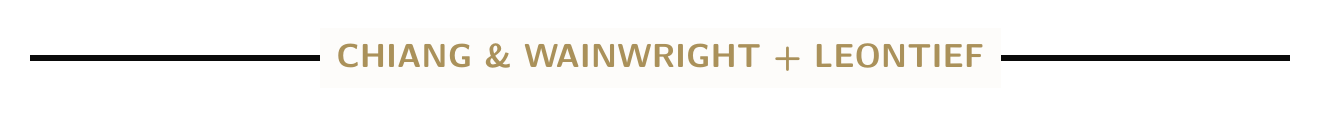
\begin{tikzpicture}
        \draw[line width=2pt, VogueBlack] (0,0) -- (16,0);
        \node[fill=SoftLinen, inner sep=6pt, text=GoldLeaf] at (8,0) {\large\textsf{\textbf{CHIANG \& WAINWRIGHT + LEONTIEF}}};
    \end{tikzpicture}
\end{center}

\begin{multicols*}{3}

% ========================================
% SECCIÓN I: NOTACIÓN MATRICIAL
% ========================================

\section{I. Notación Matricial $\mathbf{Ax = d}$}

\noindent\textbf{LA REPRESENTACIÓN FUNDAMENTAL.} Un sistema de $m$ ecuaciones lineales en $n$ variables se expresa de manera compacta como:

\begin{equation}
\mathbf{Ax = d}
\end{equation}

\subsection{Componentes del Sistema}

\begin{definitionbox}[title=Matriz de Coeficientes ($\mathbf{A}$)]
\small Arreglo rectangular $m \times n$ que contiene los coeficientes $a_{ij}$:
\begin{equation}
\mathbf{A} = \begin{bmatrix}
a_{11} & a_{12} & \cdots & a_{1n} \\
a_{21} & a_{22} & \cdots & a_{2n} \\
\vdots & \vdots & \ddots & \vdots \\
a_{m1} & a_{m2} & \cdots & a_{mn}
\end{bmatrix}_{m \times n}
\end{equation}
\end{definitionbox}

\begin{definitionbox}[title=Vector de Variables ($\mathbf{x}$)]
\small Vector columna $n \times 1$ de las incógnitas:
\begin{equation}
\mathbf{x} = \begin{bmatrix} x_1 \\ x_2 \\ \vdots \\ x_n \end{bmatrix}_{n \times 1}
\end{equation}
\end{definitionbox}

\begin{definitionbox}[title=Vector de Constantes ($\mathbf{d}$)]
\small Vector columna $m \times 1$ de términos independientes:
\begin{equation}
\mathbf{d} = \begin{bmatrix} d_1 \\ d_2 \\ \vdots \\ d_m \end{bmatrix}_{m \times 1}
\end{equation}
\end{definitionbox}

\subsection{Visualización 3D Animada: Transformación Lineal}

\noindent
\begin{animateinline}[controls, loop, autoplay]{12}
\multiframe{40}{rAngle=0+9}{%
    \tdplotsetmaincoords{70}{110}%
    \begin{tikzpicture}[tdplot_main_coords, scale=2.8]

        % Grid de referencia
        \foreach \i in {-1,-0.5,0,0.5,1} {
            \draw[SlateGrey!20, ultra thin] (\i,-1,0) -- (\i,1,0);
            \draw[SlateGrey!20, ultra thin] (-1,\i,0) -- (1,\i,0);
        }

        % Transformación dinámica
        \pgfmathsetmacro{\scaleZ}{0.7 + 0.4*sin(\rAngle)}
        \pgfmathsetmacro{\shearX}{0.25*cos(\rAngle)}

        % Plano transformado
        \fill[MITCrimson, opacity=0.12] (-1,-1,0) -- (1,-1,0) -- (1,1,{\shearX}) -- (-1,1,{\shearX}) -- cycle;

        % Vectores base
        \draw[->, >=stealth, VogueBlack, thick] (0,0,0) -- (1,0,0) node[anchor=north east, font=\tiny] {$\mathbf{e}_1$};
        \draw[->, >=stealth, VogueBlack, thick] (0,0,0) -- (0,1,0) node[anchor=north west, font=\tiny] {$\mathbf{e}_2$};

        % Vector transformado dinámico
        \draw[->, >=stealth, GoldLeaf, ultra thick] (0,0,0) -- ({\shearX}, 0.5, {\scaleZ})
            node[anchor=south, font=\tiny\bfseries] {$\mathbf{Ax}$};

        % Datos técnicos
        \node[VogueBlack, anchor=north west, font=\tiny\ttfamily] at (-1.1, 1.3, 1) {
            $\det(\mathbf{A}) = $ \pgfmathparse{\scaleZ}\pgfmathprintnumber[fixed, precision=2]{\pgfmathresult}
        };

        % Ejes 3D
        \draw[->, SlateGrey!60, thin] (0,0,0) -- (1.3,0,0);
        \draw[->, SlateGrey!60, thin] (0,0,0) -- (0,1.3,0);
        \draw[->, SlateGrey!60, thin] (0,0,0) -- (0,0,1.3);
    \end{tikzpicture}%
}
\end{animateinline}

\noindent\textbf{Interpretación Geométrica:} La animación muestra cómo una transformación lineal $\mathbf{A}$ distorsiona el espacio vectorial, preservando el origen.

% ========================================
% SECCIÓN II: DETERMINANTES
% ========================================

\section{II. Determinantes y No Singularidad}

\noindent\textbf{EL ESCALAR CARACTERÍSTICO.} El determinante $|\mathbf{A}|$ es un número que determina la invertibilidad de una matriz cuadrada.

\subsection{Definición Formal}

\begin{definitionbox}[title=Determinante]
\small Para una matriz $\mathbf{A}$ de $n \times n$:
\begin{equation}
|\mathbf{A}| = \sum_{\sigma \in S_n} \text{sgn}(\sigma) \prod_{i=1}^{n} a_{i,\sigma(i)}
\end{equation}
donde $S_n$ son todas las permutaciones de $\{1,2,\ldots,n\}$ y $\text{sgn}(\sigma)$ es el signo de la permutación.
\end{definitionbox}

\subsection{Expansión de Laplace}

\noindent\textbf{MÉTODO PRÁCTICO.} El determinante se calcula por cofactores:

\begin{theorembox}[title=Expansión por Cofactores]
\small Por el $i$-ésimo renglón:
\begin{equation}
|\mathbf{A}| = \sum_{j=1}^{n} a_{ij}|C_{ij}|
\end{equation}
Por la $j$-ésima columna:
\begin{equation}
|\mathbf{A}| = \sum_{i=1}^{n} a_{ij}|C_{ij}|
\end{equation}
donde $|C_{ij}| = (-1)^{i+j}|M_{ij}|$ es el cofactor.
\end{theorembox}

\subsection{Visualización Animada: Determinante como Volumen}

\noindent
\begin{animateinline}[controls, loop, autoplay]{10}
\multiframe{36}{iAngle=0+10}{%
    \tdplotsetmaincoords{65}{30+\iAngle}%
    \begin{tikzpicture}[tdplot_main_coords, scale=2.5]

        % Vectores columna de la matriz
        \coordinate (A) at (2.5,0.6,0);
        \coordinate (B) at (0.5,2.2,0);
        \coordinate (C) at (0.3,0.4,1.8);

        % Paralelepípedo (volumen = |det A|)
        \fill[nasablue, opacity=0.15] (0,0,0) -- (A) -- ($(A)+(B)$) -- (B) -- cycle;
        \fill[MITCrimson, opacity=0.15] (0,0,0) -- (A) -- ($(A)+(C)$) -- (C) -- cycle;
        \fill[GoldLeaf, opacity=0.15] (0,0,0) -- (B) -- ($(B)+(C)$) -- (C) -- cycle;

        % Vectores
        \draw[->, ultra thick, MITCrimson] (0,0,0) -- (A) node[midway, below] {\tiny $\mathbf{a}_1$};
        \draw[->, ultra thick, GoldLeaf] (0,0,0) -- (B) node[midway, left] {\tiny $\mathbf{a}_2$};
        \draw[->, ultra thick, nasablue] (0,0,0) -- (C) node[midway, left] {\tiny $\mathbf{a}_3$};

        % Ejes de referencia
        \draw[->, SlateGrey!40] (0,0,0) -- (3,0,0) node[right, font=\tiny] {$x$};
        \draw[->, SlateGrey!40] (0,0,0) -- (0,3,0) node[above, font=\tiny] {$y$};
        \draw[->, SlateGrey!40] (0,0,0) -- (0,0,2.5) node[above, font=\tiny] {$z$};

        % Etiqueta de volumen
        \node[VogueBlack, font=\scriptsize] at (1.2,1.2,0.9) {$V = |\det(\mathbf{A})|$};
    \end{tikzpicture}%
}
\end{animateinline}

\noindent\textbf{Fórmula Explícita 2×2:}
\begin{equation}
\begin{vmatrix} a & b \\ c & d \end{vmatrix} = ad - bc
\end{equation}

\subsection{Propiedades Críticas}

\begin{voguebox}[title=Propiedades del Determinante]
\small
\begin{enumerate}
    \item $|\mathbf{I}| = 1$ (matriz identidad)
    \item $|\mathbf{A}^T| = |\mathbf{A}|$ (transpuesta)
    \item $|\mathbf{AB}| = |\mathbf{A}||\mathbf{B}|$ (producto)
    \item $|\alpha\mathbf{A}| = \alpha^n|\mathbf{A}|$ (escalar, matriz $n \times n$)
    \item $|\mathbf{A}^{-1}| = \dfrac{1}{|\mathbf{A}|}$ (inversa)
    \item Si dos filas/columnas son iguales: $|\mathbf{A}| = 0$
    \item Intercambiar filas/columnas: $|\mathbf{A}'| = -|\mathbf{A}|$
\end{enumerate}
\end{voguebox}

% ========================================
% SECCIÓN VI: MODELO DE LEONTIEF EXPANDIDO
% ========================================

\section{VI. Modelo Input-Output de Leontief}

\noindent\textbf{ECONOMÍA INTERRELACIONADA.} Modelo que captura interdependencias productivas.

\subsection{Supuestos Fundamentales}

\begin{enumerate}
    \item Cada industria produce un producto \textbf{homogéneo}
    \item \textbf{Proporciones de insumo fijas} (coeficientes técnicos constantes)
    \item \textbf{Rendimientos constantes a escala}
\end{enumerate}

\subsection{Matriz de Coeficientes Técnicos}

\begin{definitionbox}[title=Coeficiente $a_{ij}$]
\small Unidades del producto $i$ necesarias para producir una unidad del producto $j$:
\begin{equation}
a_{ij} = \frac{\text{Insumo de } i \text{ usado por } j}{\text{Producción total de } j}
\end{equation}
\textbf{Restricción:} $\sum_{i=1}^{n} a_{ij} < 1$ (viabilidad económica)
\end{definitionbox}

\subsection{Ecuación de Balance}

\noindent La producción total satisface:
\begin{equation}
\mathbf{x} = \mathbf{Ax} + \mathbf{d}
\end{equation}

\noindent donde:
\begin{itemize}
    \item $\mathbf{x}$: vector de producción total
    \item $\mathbf{Ax}$: consumo intermedio (insumos)
    \item $\mathbf{d}$: demanda final (exógena)
\end{itemize}

\subsection{Solución del Modelo}

\begin{theorembox}[title=Fórmula de Leontief]
\small Si $(\mathbf{I} - \mathbf{A})$ es no singular:
\begin{equation}
\mathbf{x} = (\mathbf{I} - \mathbf{A})^{-1}\mathbf{d}
\end{equation}
La matriz $(\mathbf{I} - \mathbf{A})^{-1}$ es la \textbf{matriz de Leontief} o \textbf{multiplicador}.
\end{theorembox}

\subsection{Interpretación de Multiplicadores}

\begin{voguebox}[title=Multiplicador de Leontief]
\small
El elemento $(i,j)$ de la matriz inversa representa:
\begin{equation}
[(\mathbf{I} - \mathbf{A})^{-1}]_{ij} = \frac{\partial x_i}{\partial d_j}
\end{equation}
Indica cuánto debe aumentar la producción del sector $i$ cuando la demanda final del sector $j$ aumenta en una unidad.
\end{voguebox}

\subsection{Ejemplo: Economía 2 Sectores}

\noindent\textbf{Matriz tecnológica:}
\begin{equation}
\mathbf{A} = \begin{bmatrix} 0.3 & 0.2 \\ 0.1 & 0.4 \end{bmatrix}, \quad
\mathbf{d} = \begin{bmatrix} 100 \\ 50 \end{bmatrix}
\end{equation}

\noindent\textbf{Cálculo:}
\begin{align}
\mathbf{I} - \mathbf{A} &= \begin{bmatrix} 0.7 & -0.2 \\ -0.1 & 0.6 \end{bmatrix} \\
|(\mathbf{I} - \mathbf{A})| &= 0.40 \\
(\mathbf{I} - \mathbf{A})^{-1} &= \begin{bmatrix} 1.5 & 0.5 \\ 0.25 & 1.75 \end{bmatrix}
\end{align}

\noindent\textbf{Producción necesaria:}
\begin{equation}
\mathbf{x} = \begin{bmatrix} 1.5 & 0.5 \\ 0.25 & 1.75 \end{bmatrix}\begin{bmatrix} 100 \\ 50 \end{bmatrix} = \begin{bmatrix} 175 \\ 112.5 \end{bmatrix}
\end{equation}

\noindent\textbf{Interpretación:}
\begin{itemize}
    \item Si $d_1 \uparrow$ 1: $x_1 \uparrow$ 1.5, $x_2 \uparrow$ 0.25
    \item Si $d_2 \uparrow$ 1: $x_1 \uparrow$ 0.5, $x_2 \uparrow$ 1.75
\end{itemize}

\subsection{Visualización Animada: Flujo Circular Económico}

\noindent
\begin{animateinline}[controls, loop, autoplay]{8}
\multiframe{32}{rFlow=0+11.25}{%
    \begin{tikzpicture}[scale=1]
        % Sectores
        \node[circle, draw=MITCrimson, thick, fill=MITCrimson!10, minimum size=1.5cm, font=\small] (S1) at (0,0) {Sector 1};
        \node[circle, draw=GoldLeaf, thick, fill=GoldLeaf!10, minimum size=1.5cm, font=\small] (S2) at (4,0) {Sector 2};
        \node[rectangle, draw=SlateGrey, thick, fill=SlateGrey!10, minimum width=1.8cm, font=\small] (D) at (2,-3.2) {Demanda\\Final};

        % Flujos animados (opacidad variable)
        \pgfmathsetmacro{\opacityOne}{0.3 + 0.7*abs(sin(\rFlow))}
        \pgfmathsetmacro{\opacityTwo}{0.3 + 0.7*abs(cos(\rFlow))}

        % Flujos intersectoriales
        \draw[->, very thick, MITCrimson, opacity=\opacityOne] (S1) to[out=30, in=150] node[above, font=\tiny] {$a_{12}x_2$} (S2);
        \draw[->, very thick, GoldLeaf, opacity=\opacityTwo] (S2) to[out=210, in=-30] node[below, font=\tiny] {$a_{21}x_1$} (S1);

        % Autoconsumo
        \draw[->, thick, MITCrimson!60, opacity=\opacityOne] (S1) to[out=135, in=225, looseness=8] node[left, font=\tiny] {$a_{11}x_1$} (S1);
        \draw[->, thick, GoldLeaf!60, opacity=\opacityTwo] (S2) to[out=45, in=-45, looseness=8] node[right, font=\tiny] {$a_{22}x_2$} (S2);

        % Flujos a demanda final
        \draw[->, very thick, VogueBlack, opacity=\opacityOne] (S1) to node[left, font=\tiny] {$d_1=100$} (D);
        \draw[->, very thick, VogueBlack, opacity=\opacityTwo] (S2) to node[right, font=\tiny] {$d_2=50$} (D);

        % Producción total
        \node[above, font=\scriptsize, MITCrimson] at (S1.north) {$x_1 = 175$};
        \node[above, font=\scriptsize, GoldLeaf] at (S2.north) {$x_2 = 112.5$};
    \end{tikzpicture}%
}
\end{animateinline}

\subsection{Condiciones de Hawkins-Simon}

\begin{theorembox}[title=Viabilidad Económica]
\small Para que el modelo sea productivo (solución $\mathbf{x} > 0$):

\textbf{Condición suficiente:} Todos los menores principales de $(\mathbf{I} - \mathbf{A})$ son positivos.

Para $2 \times 2$:
\begin{align}
1 - a_{11} &> 0 \\
(1 - a_{11})(1 - a_{22}) - a_{12}a_{21} &> 0
\end{align}
\end{theorembox}

% ========================================
% SECCIÓN IV: REGLA DE CRAMER
% ========================================

\section{IV. Regla de Cramer}

\noindent\textbf{SOLUCIÓN ANALÍTICA.} Método para resolver $\mathbf{Ax = d}$ cuando $\mathbf{A}$ es cuadrada y no singular.

\begin{theorembox}[title=Regla de Cramer]
\small Para un sistema $\mathbf{Ax = d}$ con $|\mathbf{A}| \neq 0$, la solución es:
\begin{equation}
x_j = \frac{|\mathbf{A}_j|}{|\mathbf{A}|}
\end{equation}
donde $|\mathbf{A}_j|$ es el determinante de la matriz obtenida al reemplazar la columna $j$ de $\mathbf{A}$ por el vector $\mathbf{d}$.
\end{theorembox}

\subsection{Derivación mediante Inversión}

\noindent La solución $\mathbf{x} = \mathbf{A}^{-1}\mathbf{d}$ se expande usando $\mathbf{A}^{-1} = \frac{1}{|\mathbf{A}|}\mathbf{A}^\#$:

\begin{equation}
x_j = \frac{1}{|\mathbf{A}|} \sum_{i=1}^{n} d_i |C_{ij}| = \frac{|\mathbf{A}_j|}{|\mathbf{A}|}
\end{equation}

\noindent donde $\sum_{i=1}^{n} d_i |C_{ij}|$ es la expansión de Laplace de $|\mathbf{A}_j|$.

\subsection{Ejemplo Completo: Sistema 2×2}

\begin{equation}
\begin{cases}
2x + y = 8 \\
x - y = 1
\end{cases}
\end{equation}

\noindent\textbf{Solución:}
\begin{align}
|\mathbf{A}| &= \begin{vmatrix} 2 & 1 \\ 1 & -1 \end{vmatrix} = -3 \\
x &= \frac{\begin{vmatrix} 8 & 1 \\ 1 & -1 \end{vmatrix}}{-3} = \frac{-9}{-3} = 3 \\
y &= \frac{\begin{vmatrix} 2 & 8 \\ 1 & 1 \end{vmatrix}}{-3} = \frac{-6}{-3} = 2
\end{align}

\subsection{Visualización: Reemplazo de Columnas}

\begin{center}
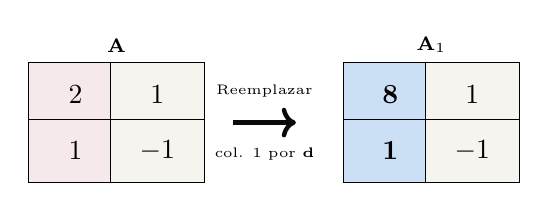
\begin{tikzpicture}[scale=0.8]
    % Matriz original
    \node[draw, minimum width=1.2cm, minimum height=0.8cm, fill=MITCrimson!10] at (0,0) {$2$};
    \node[draw, minimum width=1.2cm, minimum height=0.8cm, fill=GoldLeaf!10] at (1.3,0) {$1$};
    \node[draw, minimum width=1.2cm, minimum height=0.8cm, fill=MITCrimson!10] at (0,-0.9) {$1$};
    \node[draw, minimum width=1.2cm, minimum height=0.8cm, fill=GoldLeaf!10] at (1.3,-0.9) {$-1$};
    \node[above, font=\scriptsize] at (0.65,0.5) {$\mathbf{A}$};

    % Flecha
    \draw[->, ultra thick, VogueBlack] (2.5,-0.45) -- (3.5,-0.45);
    \node[above, font=\tiny] at (3,-0.2) {Reemplazar};
    \node[below, font=\tiny] at (3,-0.7) {col. 1 por $\mathbf{d}$};

    % Matriz A_1
    \node[draw, minimum width=1.2cm, minimum height=0.8cm, fill=nasablue!20] at (5,0) {$\mathbf{8}$};
    \node[draw, minimum width=1.2cm, minimum height=0.8cm, fill=GoldLeaf!10] at (6.3,0) {$1$};
    \node[draw, minimum width=1.2cm, minimum height=0.8cm, fill=nasablue!20] at (5,-0.9) {$\mathbf{1}$};
    \node[draw, minimum width=1.2cm, minimum height=0.8cm, fill=GoldLeaf!10] at (6.3,-0.9) {$-1$};
    \node[above, font=\scriptsize] at (5.65,0.5) {$\mathbf{A}_1$};
\end{tikzpicture}
\end{center}

% ========================================
% SECCIÓN V: EQUILIBRIO DE MERCADO
% ========================================

\section{V. Equilibrio de Mercado (2 Bienes)}

\noindent\textbf{MODELO DE EQUILIBRIO GENERAL.} Análisis de mercados interdependientes.

\subsection{Condición de Equilibrio}

\begin{definitionbox}[title=Equilibrio de Mercado]
\small El equilibrio se alcanza cuando:
\begin{equation}
q_{d_i} = q_{s_i} \quad \forall i
\end{equation}
Para cada bien $i$, la cantidad demandada iguala la cantidad ofrecida.
\end{definitionbox}

\subsection{Clasificación de Bienes}

\begin{voguebox}[title=Criterio de Efectos Cruzados]
\small Sean dos bienes con funciones de demanda que incluyen precios cruzados:
\begin{itemize}
    \item \textbf{Sustitutos:} Si $\dfrac{\partial q_{d_i}}{\partial p_j} > 0$ \\
    (↑ precio del bien $j$ $\Rightarrow$ ↑ demanda del bien $i$)
    \item \textbf{Complementos:} Si $\dfrac{\partial q_{d_i}}{\partial p_j} < 0$ \\
    (↑ precio del bien $j$ $\Rightarrow$ ↓ demanda del bien $i$)
\end{itemize}
\end{voguebox}

\subsection{Visualización Animada: Curvas de Oferta y Demanda}

\noindent
\begin{animateinline}[controls, loop, autoplay]{8}
\multiframe{24}{rShift=0+15}{%
    \begin{tikzpicture}[scale=0.65]
        % Ejes
        \draw[->, thick, SlateGrey!60] (0,0) -- (6,0) node[right, font=\tiny] {$q$};
        \draw[->, thick, SlateGrey!60] (0,0) -- (0,6) node[above, font=\tiny] {$p$};

        % Desplazamiento dinámico de demanda
        \pgfmathsetmacro{\shift}{0.5*sin(\rShift)}

        % Curva de oferta (fija)
        \draw[ultra thick, GoldLeaf, domain=0.5:5.5] plot (\x, {0.5*\x + 0.5}) node[right, font=\tiny] {$S$};

        % Curva de demanda (desplazándose)
        \draw[ultra thick, MITCrimson, domain=0.5:5.5] plot (\x, {-0.5*\x + 5 + \shift}) node[left, font=\tiny] {$D$};

        % Punto de equilibrio
        \pgfmathsetmacro{\qeq}{(4.5 + \shift)}
        \pgfmathsetmacro{\peq}{0.5*\qeq + 0.5}
        \filldraw[VogueBlack] (\qeq,\peq) circle (2.5pt);

        % Líneas punteadas
        \draw[dashed, SlateGrey!40] (\qeq,0) node[below, font=\tiny] {$q^*$} -- (\qeq,\peq);
        \draw[dashed, SlateGrey!40] (0,\peq) node[left, font=\tiny] {$p^*$} -- (\qeq,\peq);

        % Etiqueta
        \node[VogueBlack, font=\scriptsize] at (3,-1) {Equilibrio Dinámico};
    \end{tikzpicture}%
}
\end{animateinline}

\subsection{Ejemplo: Sistema 2×2}

\noindent\textbf{Funciones:}
\begin{align}
q_{d_1} &= 53 - 2p_1 - 3p_2, \quad q_{s_1} = -4 + 3p_1 \\
q_{d_2} &= 64 - 3p_1 - 4p_2, \quad q_{s_2} = -8 + 2p_2
\end{align}

\noindent\textbf{Sistema en equilibrio:}
\begin{equation}
\begin{bmatrix} 5 & 3 \\ 3 & 6 \end{bmatrix}
\begin{bmatrix} p_1 \\ p_2 \end{bmatrix}
= \begin{bmatrix} 57 \\ 72 \end{bmatrix}
\end{equation}

\noindent\textbf{Solución:}
\begin{align}
|\mathbf{A}| &= 21 \\
p_1^* &= 6, \quad p_2^* = 9 \\
q_1^* &= 14, \quad q_2^* = 10
\end{align}

\noindent\textbf{Relación:} Bienes \textbf{complementos} ($\partial q_{d_1}/\partial p_2 = -3 < 0$)

% ========================================
% SECCIÓN VII: MODELO DE RENTA NACIONAL
% ========================================

\section{VII. Modelo Simple de Renta Nacional}

\noindent\textbf{MODELO KEYNESIANO.} Determinación del ingreso de equilibrio.

\subsection{Variables y Ecuaciones}

\begin{definitionbox}[title=Estructura del Modelo]
\small
\textbf{Variables Endógenas:} $Y$ (Renta Nacional), $C$ (Consumo)

\textbf{Variables Exógenas:} $I_0$ (Inversión), $G_0$ (Gasto Público)

\textbf{Ecuaciones:}
\begin{align}
Y &= C + I_0 + G_0 \quad \text{(Identidad contable)} \\
C &= \alpha + \beta Y \quad \text{(Función de consumo)}
\end{align}

\textbf{Parámetros:}
\begin{itemize}
    \item $\alpha > 0$: Consumo autónomo
    \item $\beta \in (0,1)$: Propensión marginal a consumir (PMC)
    \item $s = 1-\beta$: Propensión marginal a ahorrar
\end{itemize}
\end{definitionbox}

\subsection{Solución Matricial}

\noindent\textbf{Forma matricial $\mathbf{Ax = d}$:}
\begin{equation}
\begin{bmatrix} 1 & -1 \\ -\beta & 1 \end{bmatrix}
\begin{bmatrix} Y \\ C \end{bmatrix}
= \begin{bmatrix} I_0 + G_0 \\ \alpha \end{bmatrix}
\end{equation}

\noindent\textbf{Determinante:}
\begin{equation}
|\mathbf{A}| = 1 - \beta = s > 0
\end{equation}

\subsection{Forma Reducida}

\begin{theorembox}[title=Equilibrio de Renta Nacional]
\small
\begin{align}
Y^* &= \frac{I_0 + G_0 + \alpha}{1-\beta} = \frac{I_0 + G_0 + \alpha}{s} \\
C^* &= \frac{\alpha + \beta(I_0 + G_0)}{1-\beta}
\end{align}

\textbf{Multiplicador keynesiano:}
\begin{equation}
\frac{\partial Y}{\partial I_0} = \frac{\partial Y}{\partial G_0} = \frac{1}{1-\beta} = \frac{1}{s}
\end{equation}
\end{theorembox}

\subsection{Visualización: Efecto Multiplicador}

\begin{center}
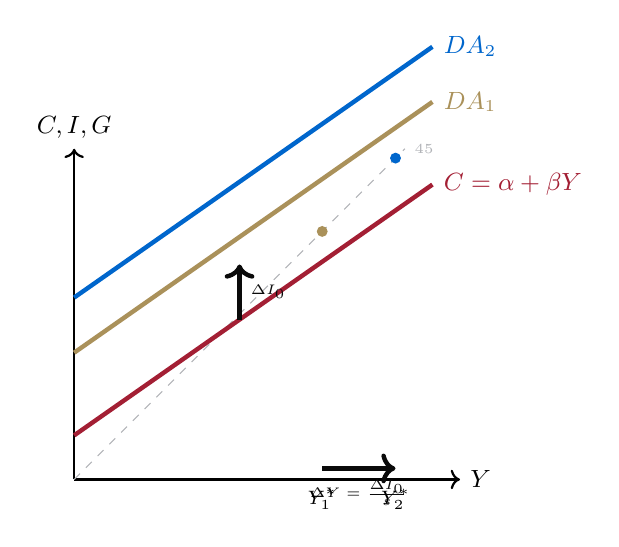
\begin{tikzpicture}[scale=0.7]
    % Ejes
    \draw[->, thick] (0,0) -- (7,0) node[right, font=\small] {$Y$};
    \draw[->, thick] (0,0) -- (0,6) node[above, font=\small] {$C,I,G$};

    % Línea 45°
    \draw[dashed, SlateGrey!40] (0,0) -- (6,6) node[right, font=\tiny] {$45°$};

    % Función de consumo
    \draw[ultra thick, MITCrimson, domain=0:6.5] plot (\x, {0.7*\x + 0.8}) node[right, font=\small] {$C = \alpha + \beta Y$};

    % Demanda agregada inicial
    \draw[ultra thick, GoldLeaf, domain=0:6.5] plot (\x, {0.7*\x + 2.3}) node[right, font=\small] {$DA_1$};

    % Demanda agregada después del shock
    \draw[ultra thick, nasablue, domain=0:6.5] plot (\x, {0.7*\x + 3.3}) node[right, font=\small] {$DA_2$};

    % Puntos de equilibrio
    \filldraw[GoldLeaf] (4.5,4.5) circle (2.5pt);
    \filldraw[nasablue] (5.83,5.83) circle (2.5pt);

    % Flechas de desplazamiento
    \draw[->, ultra thick, VogueBlack] (3,2.9) -- (3,3.9) node[midway, right, font=\tiny] {$\Delta I_0$};
    \draw[->, ultra thick, VogueBlack] (4.5,0.2) -- (5.83,0.2) node[midway, below, font=\tiny] {$\Delta Y = \frac{\Delta I_0}{s}$};

    % Etiquetas
    \node[below, font=\scriptsize] at (4.5,0) {$Y_1^*$};
    \node[below, font=\scriptsize] at (5.83,0) {$Y_2^*$};
\end{tikzpicture}
\end{center}

\noindent\textbf{Interpretación:} Un incremento en inversión $\Delta I_0$ genera un aumento amplificado en la renta $\Delta Y = \frac{\Delta I_0}{s}$ debido al efecto multiplicador.

\begin{center}
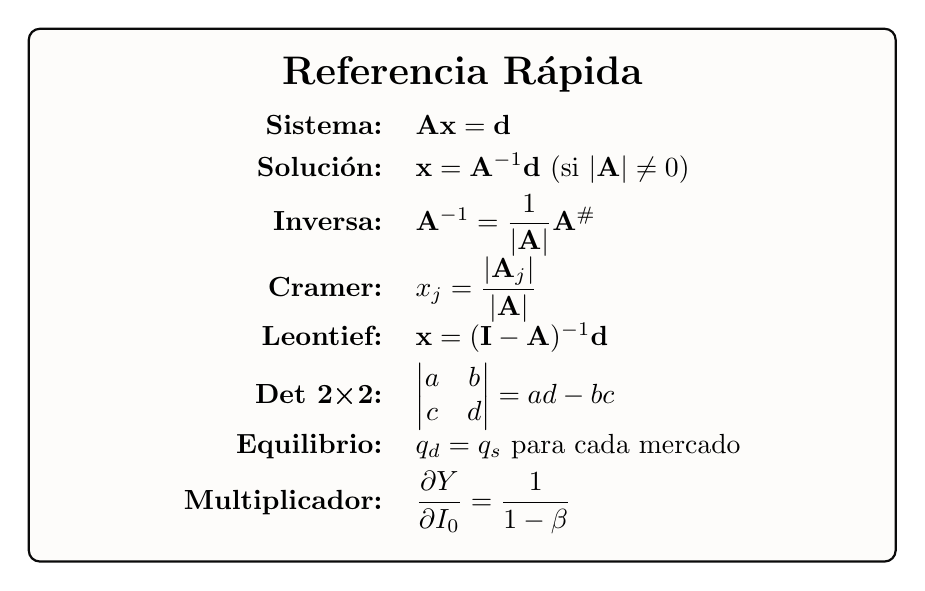
\begin{tikzpicture}
\node[draw=VogueBlack, thick, fill=SoftLinen, inner sep=10pt, rounded corners] {
\begin{minipage}{0.85\linewidth}
\centering
\textbf{\Large Referencia Rápida}

\vspace{6pt}

\begin{tabular}{rl}
\textbf{Sistema:} & $\mathbf{Ax = d}$ \\[3pt]
\textbf{Solución:} & $\mathbf{x} = \mathbf{A}^{-1}\mathbf{d}$ (si $|\mathbf{A}| \neq 0$) \\[3pt]
\textbf{Inversa:} & $\mathbf{A}^{-1} = \dfrac{1}{|\mathbf{A}|}\mathbf{A}^\#$ \\[3pt]
\textbf{Cramer:} & $x_j = \dfrac{|\mathbf{A}_j|}{|\mathbf{A}|}$ \\[3pt]
\textbf{Leontief:} & $\mathbf{x} = (\mathbf{I} - \mathbf{A})^{-1}\mathbf{d}$ \\[3pt]
\textbf{Det 2×2:} & $\begin{vmatrix} a & b \\ c & d \end{vmatrix} = ad - bc$ \\[3pt]
\textbf{Equilibrio:} & $q_d = q_s$ para cada mercado \\[3pt]
\textbf{Multiplicador:} & $\dfrac{\partial Y}{\partial I_0} = \dfrac{1}{1-\beta}$ \\
\end{tabular}
\end{minipage}
};
\end{tikzpicture}
\end{center}

\secbar

% ========================================
% SECCIÓN X: TABLA DE REFERENCIA
% ========================================

\section{X. Casos Especiales y Aplicaciones}

\begin{center}
\small
\begin{tabular}{|l|l|l|}
\hline
\textbf{Modelo} & \textbf{Característica} & \textbf{Condición Clave} \\
\hline
\hline
Equilibrio Parcial & Un mercado aislado & $q_d = q_s$ \\
\hline
Equilibrio General & $n$ mercados interdep. & Sistema $n \times n$ \\
\hline
Leontief Abierto & Sector externo & $(\mathbf{I}-\mathbf{A})$ no singular \\
\hline
Leontief Cerrado & Sin sector externo & Infinitas soluciones \\
\hline
Renta Nacional & Modelo keynesiano & $|\mathbf{A}| = 1-\beta = s$ \\
\hline
Bienes Sustitutos & $\partial q_i/\partial p_j > 0$ & Efecto cruzado + \\
\hline
Bienes Complementos & $\partial q_i/\partial p_j < 0$ & Efecto cruzado $-$ \\
\hline
\end{tabular}
\end{center}

% ========================================
% INFORMACIÓN DE CONTACTO Y AGRADECIMIENTOS
% ========================================

\section*{Agradecimientos}

\begin{voguebox}
\centering
\small
Este material educativo está dedicado a estudiantes y profesionales de economía matemática que buscan dominar el álgebra matricial aplicada.

\vspace{8pt}

Agradecemos especialmente a:
\begin{itemize}
    \item Los profesores del Departamento de Matemáticas de la \textbf{Universidad Pedagógica y Tecnológica de Colombia (UPTC)} por su invaluable guía académica en el desarrollo de este compendio
    \item La comunidad open-source de \LaTeX, TikZ y PGFPlots por proporcionar herramientas excepcionales para la divulgación científica
    \item Los autores Chiang, Wainwright y Leontief, cuyos trabajos fundamentales inspiraron esta síntesis
\end{itemize}

\vspace{10pt}

\textit{«El álgebra es generosa: a menudo da más de lo que se le pide.»} \\
\textit{«In mathematics you don't understand things. You just get used to them.»}

\vspace{4pt}

— Jean le Rond d'Alembert \& John von Neumann
\end{voguebox}

\vspace{8pt}

\begin{voguebox}
\centering

\textbf{\large Información del Autor}

\vspace{8pt}

% Línea divisoria decorativa
\rule{0.8\textwidth}{0.2pt}

\vspace{8pt}

% Información de contacto en dos columnas
\noindent\begin{minipage}[t]{0.48\textwidth}
\raggedright\footnotesize
\faIcon{envelope} \textbf{Email:}\\[2pt]
\href{mailto:emanuel.quintana@uptc.edu.co}{\small emanuel.quintana@uptc.edu.co}

\vspace{8pt}

\faIcon{id-badge} \textbf{ORCID:}\\[2pt]
\href{https://orcid.org/0009-0006-8419-2805}{\small 0009-0006-8419-2805}

\vspace{8pt}

\faIcon{university} \textbf{Institución:}\\[2pt]
{\small Universidad Pedagógica y \\Tecnológica de Colombia (UPTC)}
\end{minipage}
\hfill
\begin{minipage}[t]{0.48\textwidth}
\raggedright\footnotesize
\faIcon{github} \textbf{GitHub:}\\[2pt]
\href{https://github.com/emanuelquintana-glitch}{\small @emanuelquintana-glitch}

\vspace{8pt}

\faIcon{code-branch} \textbf{Repositorio:}\\[2pt]
\href{https://github.com/emanuelquintana-glitch/-Apuntes_Economia_Matematica.git}{\small Apuntes\_Economia\_Matematica}

\vspace{8pt}

\faIcon{book} \textbf{Programa:}\\[2pt]
{\small Economía Matemática}
\end{minipage}

\vspace{10pt}

% Línea divisoria
\rule{0.8\textwidth}{0.2pt}

\vspace{8pt}

% Estadísticas y badges
{\footnotesize
\faIcon{users} \textbf{3} seguidores ·
\faIcon{user-friends} \textbf{78} siguiendo ·
\faIcon{star} Material de referencia académica ·
\faIcon{creative-commons} CC BY-NC-SA 4.0
}

\vspace{8pt}

\textit{\small Este documento fue compilado con \LaTeX, TikZ, PGFPlots y la librería animate para visualizaciones dinámicas. El código fuente está disponible en el repositorio de GitHub bajo licencia Creative Commons.}

\vspace{5pt}
\end{voguebox}

\end{multicols*}

% --- PIE DE PÁGINA ---
\begin{tikzpicture}[remember picture, overlay]
    \draw[VogueBlack, line width=0.5pt] ($(current page.south west) + (0.5in, 0.4in)$) -- ($(current page.south east) + (-0.5in, 0.4in)$);
    \node[anchor=west] at ($(current page.south west) + (0.5in, 0.25in)$) {\tiny \textcopyright\ 2025 Emanuel Quintana Silva \textbar\ UPTC \textbar\ Economía Matemática \textbar\ Todos los derechos reservados};
    \node[anchor=east] at ($(current page.south east) + (-0.5in, 0.25in)$) {\tiny \texttt{Última actualización: Enero 2025}};
\end{tikzpicture}

\end{document}
